\section{Background}

\subsection[Why]{Malware ground truths: Why}

\begin{frame}
    \frametitle{Why do we need better malware ground truth?}
    \centering

    Malware ground truths are essential for the definition, \\
    the detection and the comprehension of Android malware

    \begin{figure}[!ht]
        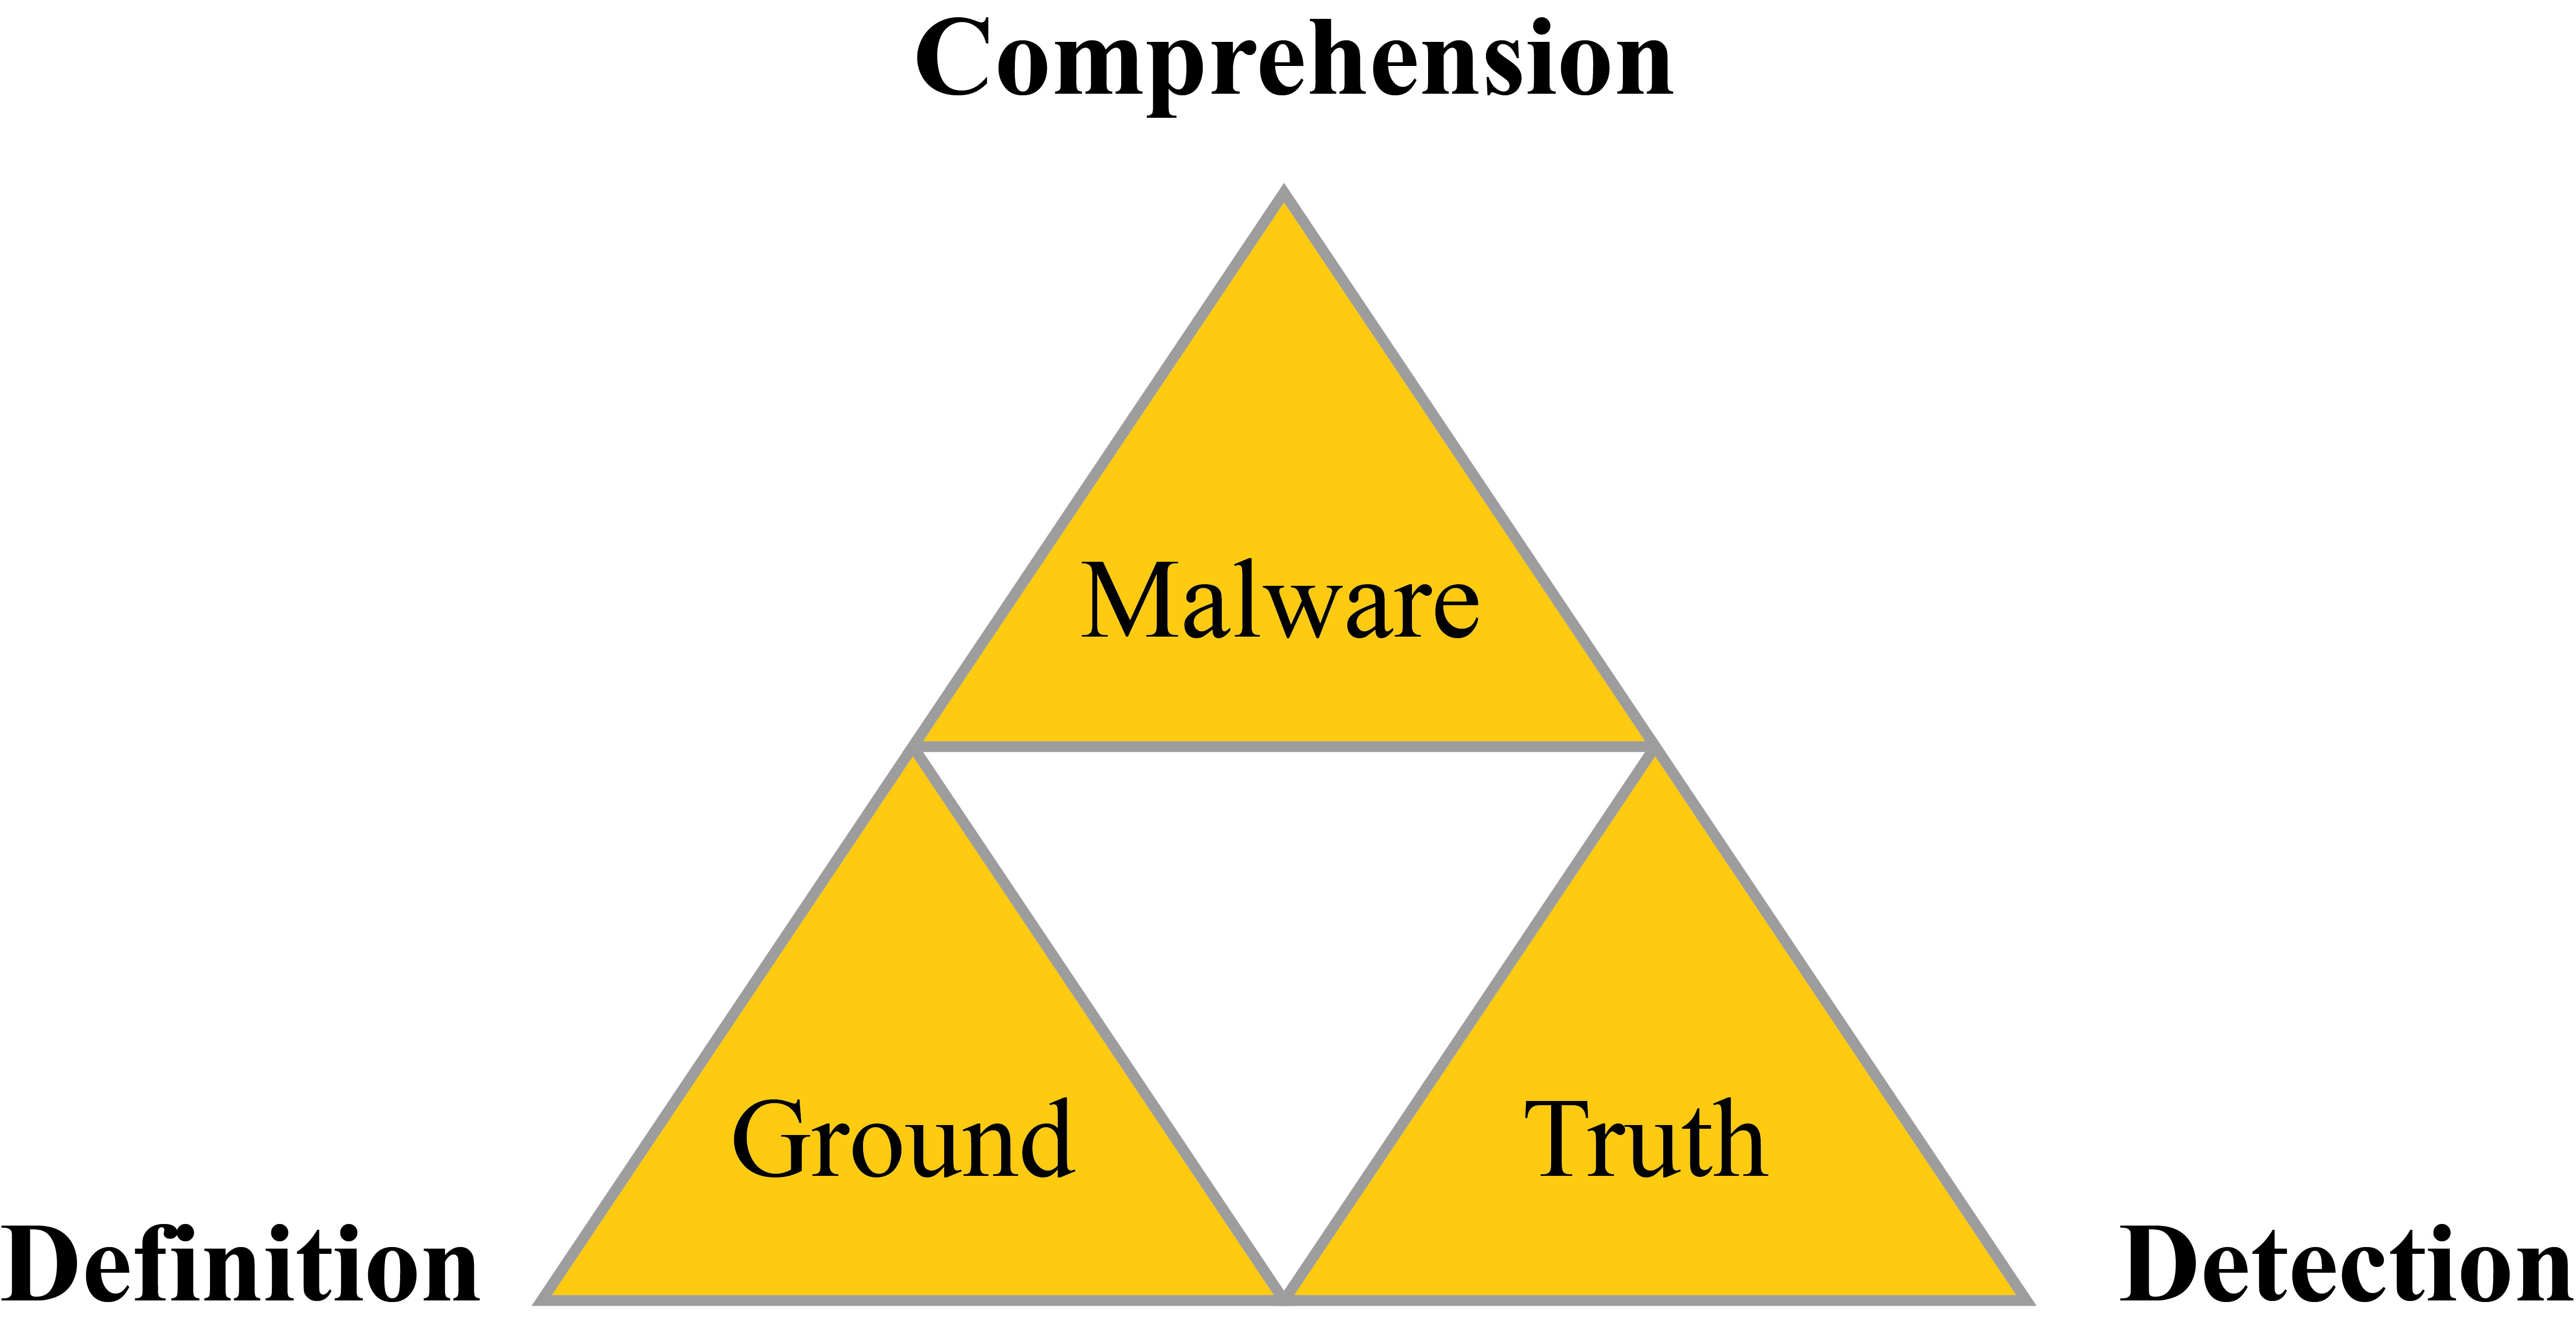
\includegraphics[width=\textwidth]{figures/background/triforce.jpg}
    \end{figure}

\end{frame}

\subsection[What]{Malware ground truths: What}

\begin{frame}
    \frametitle{What are malware ground truth in practice?}
    \centering

    \textbf{Malware ground truth} = application dataset + metadata

    \begin{table}[t]
        \resizebox{\textwidth}{!}{
            \begin{tabular}{|c|c|c|c|c|}
    \hline
    \textbf{Application ID} & \textbf{Type} & \textbf{Family} & \textbf{Variant} & Attack patterns \\
    \hline
    000000000000001 & trojan & ADRD & a & repackaging, steal information \\
    000000000000002 & backdoor & Asroot & 1 & exploit, remote control \\
    \textbf{000000000000003} & \textbf{click fraud} & \textbf{FakeNetflix} & \textbf{alpha} & \textbf{steal information} \\
    000000000000004 & rooting & Lovetrap & 201701 & exploit, privilege escalation \\
    000000000000005 & clickfraud & FakeNetflix & beta & persistence, steal information \\
    000000000000006 & trojan &  BaseBridge & 201801 & repackaging, phone calls \\
    000000000000007 & trojan & ADRD & b & repackaging, display ads \\
    000000000000008 & backdoor & Asroot & 2 & exploit, remote control  \\
    \hline
\end{tabular}

        }
        \caption{\footnotesize{Example of a malware ground truth composed of 8 malicious applications}}
    \end{table}

    Information about malware can be found in \textbf{antivirus labels}: \\
    e.g., Click-Fraud:Android/FakeNetflix.alpha

\end{frame}

\subsection[Where]{Malware ground truths: Where}

\begin{frame}
    \frametitle{Where can we find malware ground truths?}

    \begin{block}{}
        \centering
        \textbf{Datasets from research projects}
    \end{block}
    \vspace{-15pt}
    \begin{table}[t]
        \resizebox{\textwidth}{!}{
            \begin{tabular}{|c|c|c|r|r|c|}
    \hline
    \textbf{Name} & \textbf{Authors} & \textbf{Release} & \textbf{\# Samples} & \textbf{\# Families} & \textbf{Ground truth} \\
    \hline
    \textbf{Genome} & Zhou et al. [ZJ12] & 2012 & 1,260 & 49 & manual analysis \\
    \textbf{Drebin} & Arp et al. [ASH+14] & 2014 & 5,560 & 179 & supervised learning \\
    \textbf{Kharon} & Kiss et al. [KLLVTT16] & 2016 & 17 & 17 & manual analysis \\
    \textbf{Androzoo} & Allix et al. [ABKT16] & 2016 & 9,103,427 & - & VirusTotal reports \\
    \textbf{AMD} & Wei et al. [WLR+17] & 2017 & 24,650 & 71 & manual + clustering \\
    \hline
\end{tabular}

        }
    \end{table}

    \begin{block}{}
        \centering
        \textbf{Datasets from industrial projects}
    \end{block}
    \begin{table}[t]
        \resizebox{\textwidth}{!}{
            \begin{tabular}{|c|c|c|r|r|c|}
    \hline
    \textbf{Name} & \textbf{Authors} & \textbf{Release} & \textbf{\# Samples} & \textbf{\# Families} & \textbf{Ground truth} \\
    \hline
    \textbf{Contagio} & Mila Parkour [Par] & 2011 & 252 & - & manual analysis \\
    \textbf{MISP} & CIRCL [CIR] & 2012 & - & - & information sharing \\
    \textbf{Koodous} &  Koodous Project [RLVS] & 2015 & 8,314,139 & - & manual analysis \\
    \textbf{Malpedia} & Fraunhofer FKIE [Plo] & 2017 & 3,720 & 1,302 & manual analysis \\
    \hline
\end{tabular}

        }
    \end{table}

\end{frame}
